%----------------------------------------------------------------------------------------
%    PACKAGES AND THEMES
%----------------------------------------------------------------------------------------

\documentclass[aspectratio=169,xcolor=dvipsnames]{beamer}
\usetheme{SimplePlus}

\usepackage{tikz}
\usepackage{hyperref}
\usepackage{graphicx} % Allows including images
\usepackage{booktabs} % Allows the use of \toprule, \midrule and \bottomrule in tables
\usepackage{wrapfig}
\usepackage{listings}
\usepackage[font=small,labelfont=bf]{caption}

%----------------------------------------------------------------------------------------
%    TITLE PAGE
%----------------------------------------------------------------------------------------

\title{Modeling Classification}
\subtitle{HI 743}

\author{Ryan Gallagher}

\institute
{
    Department of Health Informatics and Administration \\
    Zilber College of Public Health \\
    University of Wisconsin - Milwaukee% Your institution for the title page
}
\date{February 27, 2025} % Date, can be changed to a custom date


%----------------------------------------------------------------------------------------
%    PRESENTATION SLIDES
%----------------------------------------------------------------------------------------

\begin{document}
\begin{frame}
    % Print the title page as the first slide
    \titlepage
\end{frame}

%----------------------------------------------------------------------------------------
%    Outline
%----------------------------------------------------------------------------------------

\begin{frame}{Overview}
    % Throughout your presentation, if you choose to use \section{} and \subsection{} commands, these will automatically be printed on this slide as an overview of your presentation
    \tableofcontents
\end{frame}

%----------------------------------------------------------------------------------------
%    Slides
%----------------------------------------------------------------------------------------
\section{Classification Intro}
\begin{frame}{What is Classification?}
    \textbf{Classification} is a predictive modeling task where the \textbf{response variable is categorical}.
    \begin{itemize}
        \item Unlike regression, classification predicts discrete labels instead of continuous values.
        \item Example: Predicting whether a patient has a disease (Yes/No) based on symptoms.
        \item Applications: Medical diagnosis, fraud detection, spam filtering, etc.
    \end{itemize}
    \bigskip
    \textbf{Examples of Classification Problems}:
        \begin{itemize}
        \item \textbf{Medical Diagnosis:} Does a patient have diabetes? (Yes/No)
        \item \textbf{Fraud Detection:} Is a bank transaction fraudulent? (Fraud/Not Fraud)
        \item \textbf{Genetics:} Classifying a genetic mutation as harmful or benign.
        \item \textbf{Customer Churn:} Will a customer continue using a service? (Stay/Leave)
    \end{itemize}
\end{frame}


% Slide 4: Dataset Example (ISL Default Dataset)
\begin{frame}{Example: Default Data Set}
    \textbf{Objective:} Predict whether an individual will default on a credit card payment.
    \begin{itemize}
        \item Response Variable: \texttt{Default} (Yes/No)
        \item Predictors: Income, Balance, Student Status
    \end{itemize}
    \begin{figure}
        \centering
        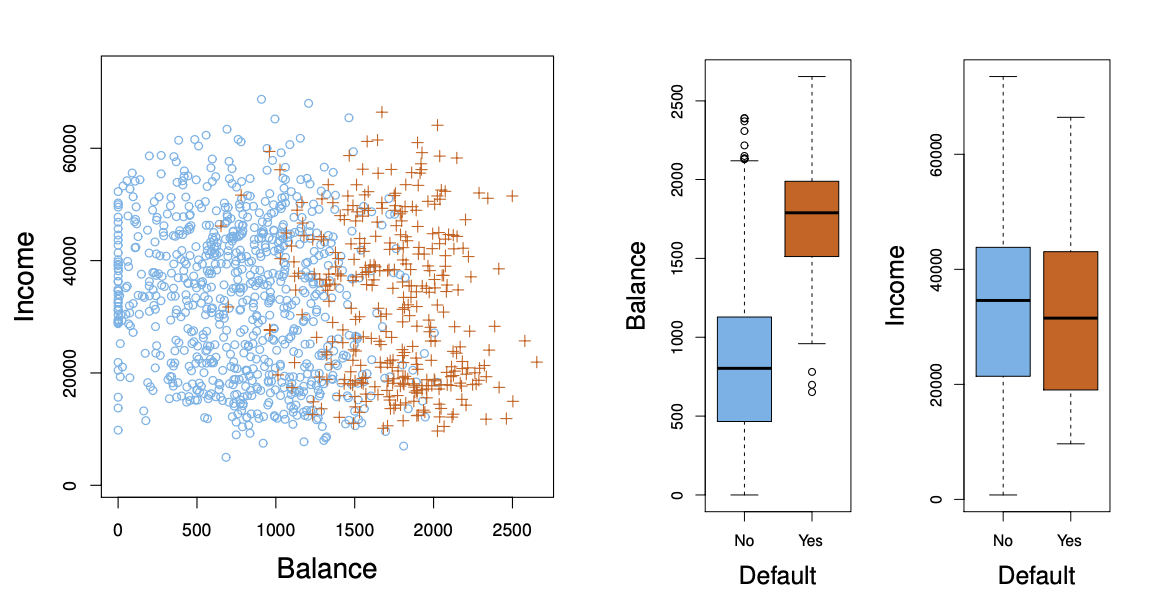
\includegraphics[width=0.6\linewidth]{images/default_data.png}
        \caption{Credit card default dataset visualization.}
    \end{figure}
\end{frame}

% Slide 5: Why Not Linear Regression?
\begin{frame}{Why Not Linear Regression?}
    \begin{itemize}
        \item Linear regression assumes a continuous response variable, making it unsuitable for predicting discrete class labels.
        \item Predictions from a linear model can extend beyond the valid probability range of \([0,1]\), which is problematic for classification.
    \end{itemize}
    \centering
    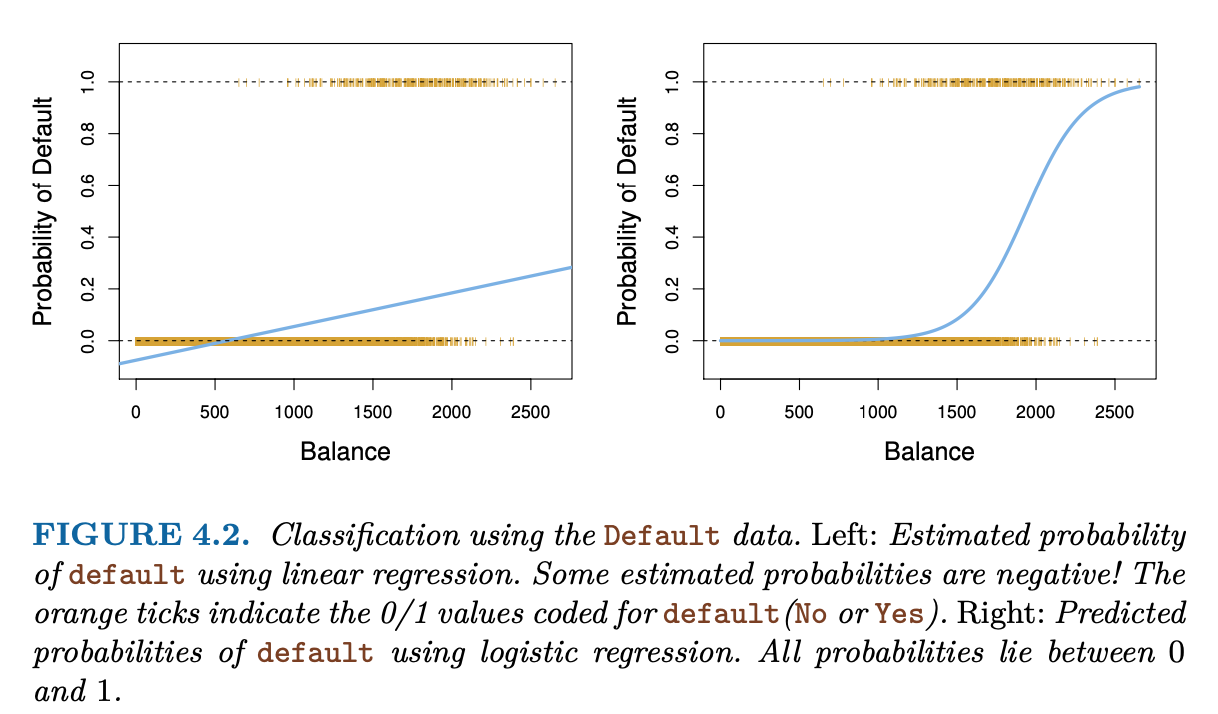
\includegraphics[width=0.6\linewidth]{images/lin_logi.png}
\end{frame}
\section{Logistic Regression}
\subsection{Logistic Regression}
% Slide 6: Logistic Regression
\begin{frame}{Logistic Regression}
\textbf{Logistic regression models the probability that a given observation belongs to a particular class.}	The logistic function ensures predictions stay within \([0,1]\):
        \begin{equation}
            P(Y=1|X) = \frac{e^{\beta_0 + \beta_1X}}{1 + e^{\beta_0 + \beta_1X}}
        \end{equation} \\
        Unlike linear regression, logistic regression predicts probabilities instead of continuous values. $P(Y=1|X)$ reads as "The probability of Y equal to 1 given X".
	\end{frame}

\begin{frame}{Logistic Regression}
	The model uses the log-odds (logit) transformation to relate predictors to the probability of an event occurring:
        \begin{equation}
            \,log \left( \frac{P(Y=1|X)}{1 - P(Y=1|X)} \right) = \beta_0 + \beta_1 X
        \end{equation}
	Maximum likelihood estimation (MLE) is used to estimate the coefficients, rather than least squares.
	The coefficients indicate how much the \textit{log-odds} of the outcome change with a one-unit increase in the predictor. 
\end{frame}

\subsection{Interpretation}
% Slide 9: Logistic Regression Interpretation
\begin{frame}{Interpreting Logistic Regression}
    \begin{itemize}
    	\setlength\itemsep{0.33cm}
        \item A positive coefficient \( \beta_1 \) implies an increase in the predictor increases the probability of the event.
        \item A negative coefficient implies a decrease in probability.
        \item The odds ratio \( e^{\beta_1} \) represents how the odds change with a one-unit increase in the predictor.
        \item Example: If \( \beta_1 = 0.3 \), then \( e^{0.3} \approx 1.35 \), meaning the odds increase by 35\%.
    \end{itemize}
    %\begin{figure}
        %\centering
        %\includegraphics[width=0.7\linewidth]{logistic_interpretation.png}
        %\caption{Interpreting coefficients in logistic regression.}
    %\end{figure}
\end{frame}

\begin{frame}{Understanding Odds and Odds Ratios}
    \begin{itemize}
        \item \textbf{Odds:} The odds of an event occurring is defined as:
        \begin{equation}
            \text{Odds} = \frac{P(Y=1)}{1 - P(Y=1)}
        \end{equation}
        \item If \( P(Y=1) = 0.75 \), then the odds are \( \frac{0.75}{0.25} = 3 \), meaning the event is three times as likely to occur than not.
    \end{itemize}
\end{frame}

\begin{frame}{Understanding Odds and Odds Ratio}
\begin{itemize}
\item \textbf{Odds Ratio (OR):} Compares the odds of an event occurring for different values of a predictor variable.
        \item The odds ratio is given by:
        \begin{equation}
            \text{OR} = \frac{P(Y=1 | X+1) / (1 - P(Y=1 | X+1))}{P(Y=1 | X) / (1 - P(Y=1 | X))}
        \end{equation}
        \item If \( OR > 1 \), the event is more likely as the predictor increases; if \( OR < 1 \), the event is less likely.
        \item Example: If \( OR = 2.5 \), the event is 2.5 times more likely for each unit increase in the predictor.
    \end{itemize}

\end{frame}

\begin{frame}{Understanding Odds and Odds Ratio}
    \begin{figure}
        \centering
        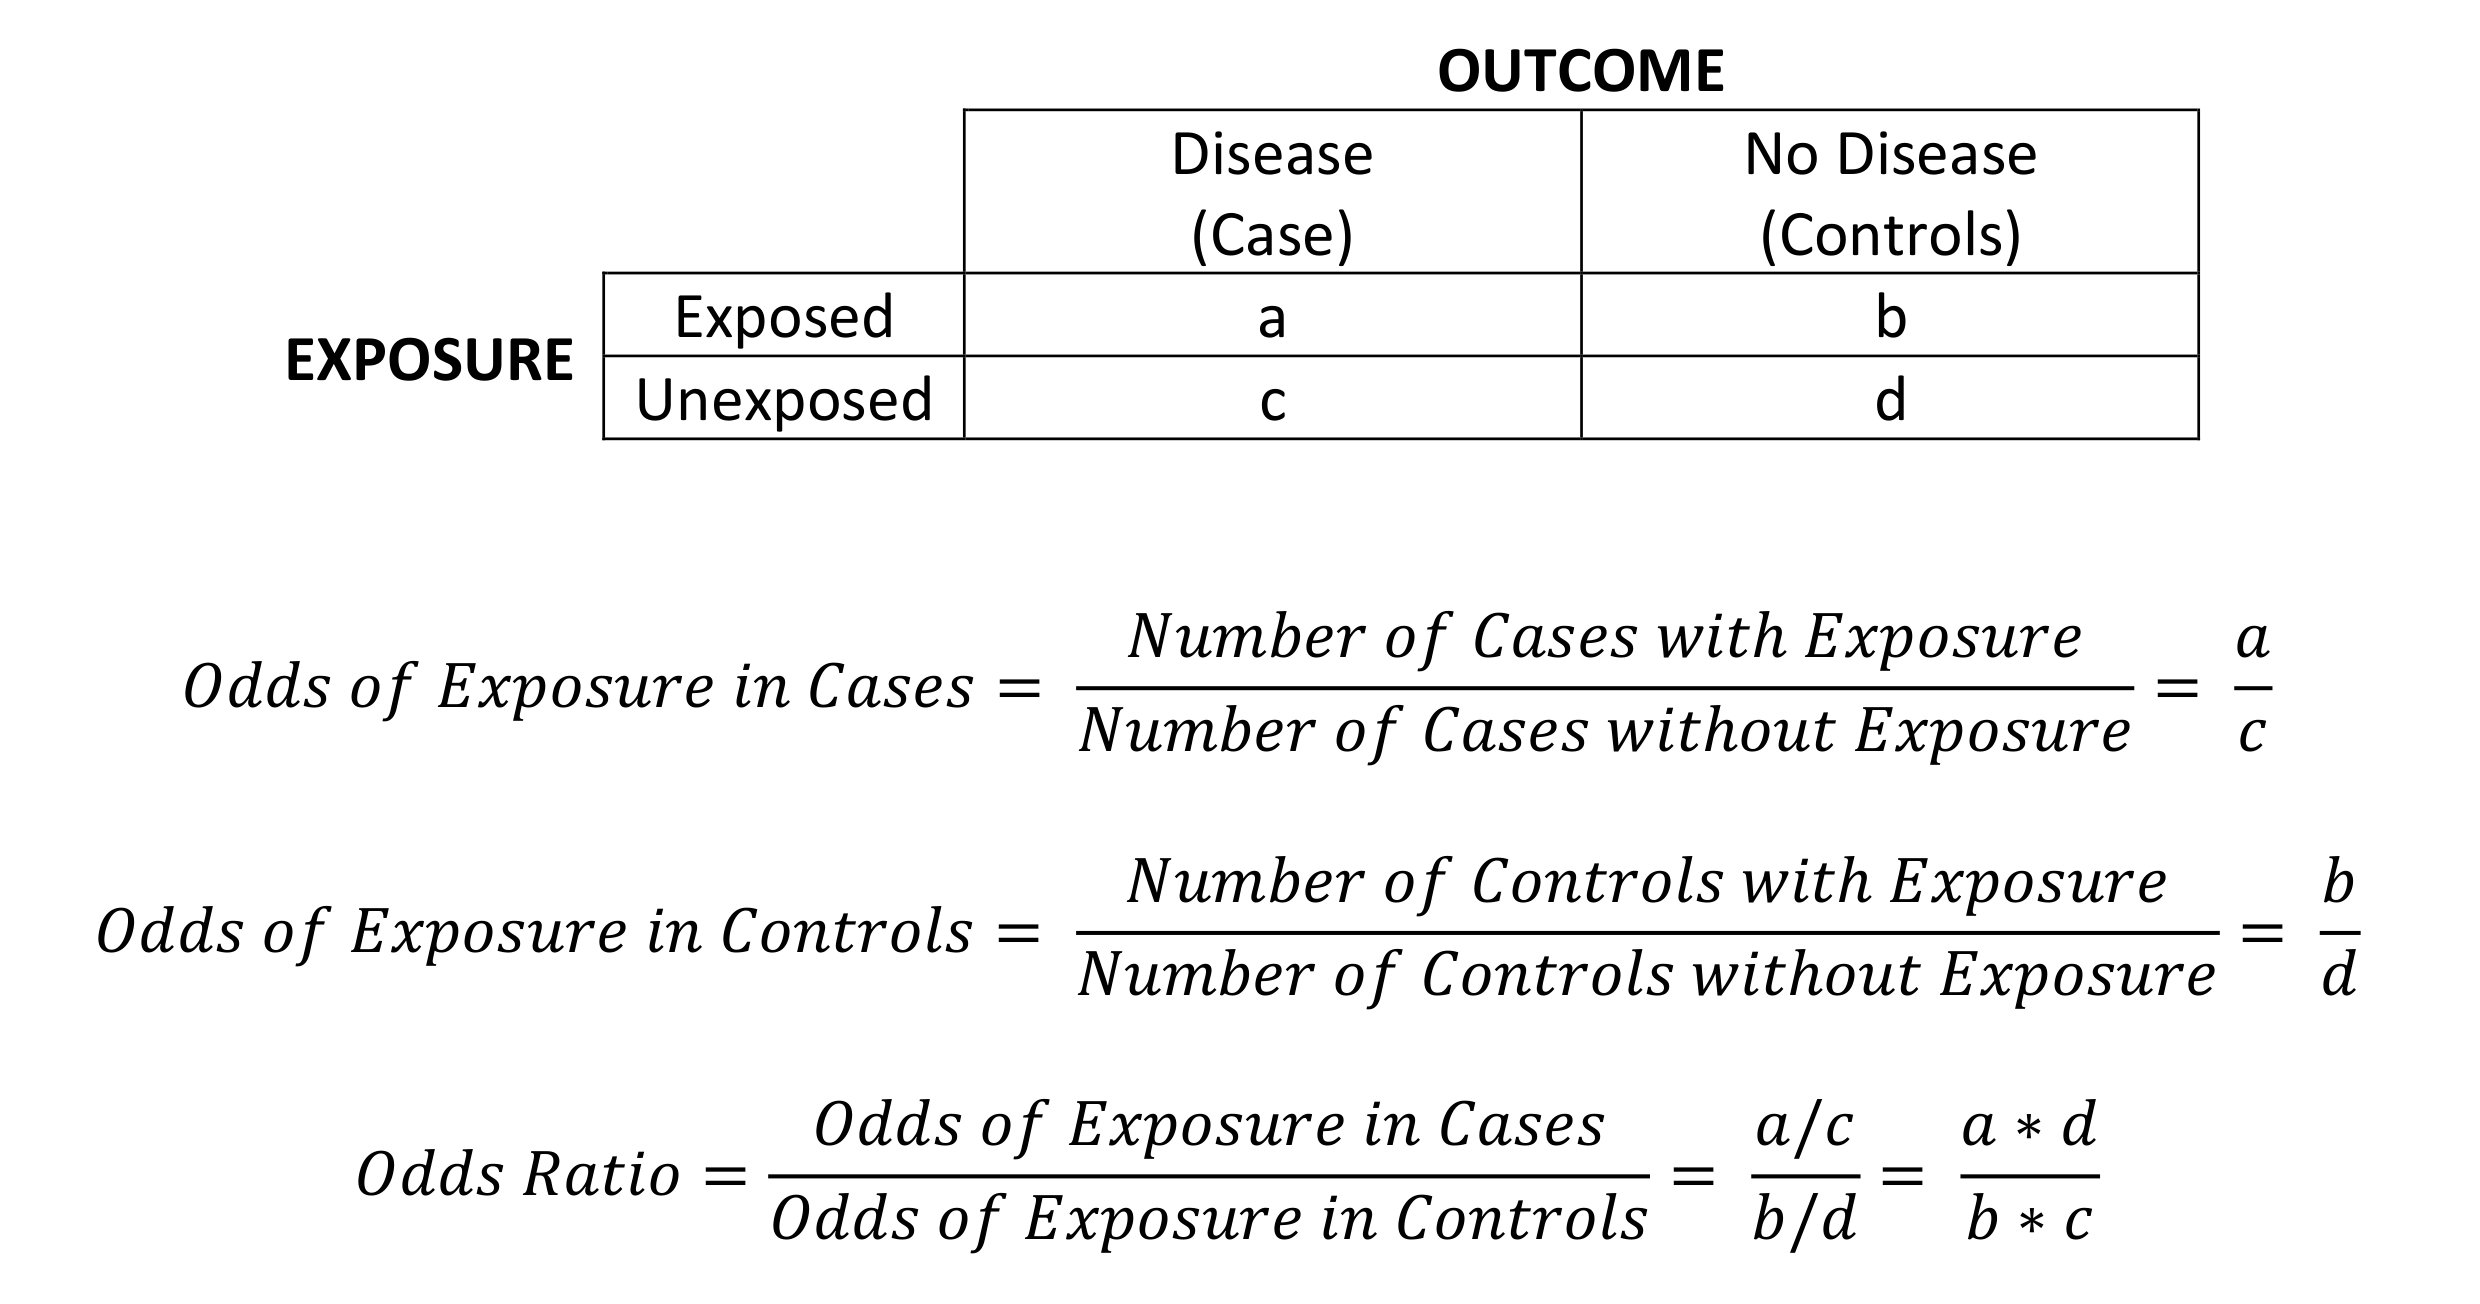
\includegraphics[width=0.8\linewidth]{images/odds_ratio.png}
    \end{figure}

\end{frame}

% Slide 12: Logistic Regression Model Output
\subsection{Output}
\begin{frame}{Logistic Regression Model Output}
    \textbf{Fitted Model:}
    \begin{equation}
        \log \left( \frac{P(Y=1 | X)}{1 - P(Y=1 | X)} \right) = -5.2 + 0.04X
    \end{equation}
    \textbf{Interpretation:}
    \begin{itemize}
        \item Intercept (\(-5.2\)): Baseline log-odds of diabetes when glucose = 0.
        \item Coefficient (\(0.04\)): A one-unit increase in glucose increases log-odds of diabetes by 0.04.
        \item Normal glucose levels range between \(70-99\), meaning individuals within this range generally have lower predicted probabilities of diabetes.
    \end{itemize}
\end{frame}

% Slide 13: Calculating Predicted Probabilities
\begin{frame}{Calculating Predicted Probabilities}
    \textbf{Example: Patient with Glucose Level = 150}
    \begin{equation}
        \text{Log-Odds} = -5.2 + (0.04 \times 150) = 0.8
    \end{equation}
    \begin{equation}
        \text{Probability} = \frac{e^{0.8}}{1 + e^{0.8}} \approx 0.69
    \end{equation}
    \textbf{Interpretation:} This patient has a 69\% probability of having diabetes.
    \begin{itemize}
        \item A patient with glucose level \(X = 85\) (mid-normal range) would have:
        \begin{equation}
            \text{Log-Odds} = -5.2 + (0.04 \times 85) = -1.8
        \end{equation}
        \begin{equation}
            \text{Probability} = \frac{e^{-1.8}}{1 + e^{-1.8}} \approx 0.14
        \end{equation}
        \item Meaning, a patient in the normal glucose range has a much lower probability of diabetes.
    \end{itemize}
\end{frame}

% Slide 14: Thresholding for Classification
\begin{frame}{Thresholding for Classification}
    \begin{itemize}
        \item A threshold (e.g., 0.5) is applied to classify patients.
        \item If \( P(Y=1 | X) > 0.5 \), classify as diabetic (\( Y=1 \)).
        \item If \( P(Y=1 | X) \leq 0.5 \), classify as non-diabetic (\( Y=0 \)).
        \item Example: With a probability of 0.69, the patient is classified as diabetic.
        \item Patients within the normal glucose range typically have probabilities well below 0.5, supporting non-diabetic classification.
    \end{itemize}
\end{frame}

\subsection{Model Evaluation}
% Slide 16: Logistic Regression Model Evaluation - Basic Metrics
\begin{frame}{Classification Model Evaluation - Basic Metrics}
    \textbf{Metrics for Evaluating Model Performance:}
    \begin{itemize}
        \item \textbf{Accuracy:} Measures the proportion of correctly classified cases.
        \begin{equation}
            \text{Accuracy} = \frac{TP + TN}{TP + TN + FP + FN}
        \end{equation}
        \item \textbf{Precision:} Measures how many predicted positives are actually correct.
        \begin{equation}
            \text{Precision} = \frac{TP}{TP + FP}
        \end{equation}
        \item \textbf{Recall (Sensitivity):} Measures how many actual positives were correctly identified.
        \begin{equation}
            \text{Recall} = \frac{TP}{TP + FN}
        \end{equation}
    \end{itemize}
\end{frame}

% Slide 17: Logistic Regression Model Evaluation - Advanced Metrics
\begin{frame}{Classification Model Evaluation - Advanced Metrics}
    \textbf{Additional Performance Measures:}
    \begin{itemize}
        \item \textbf{F1-Score:} Harmonic mean of precision and recall, balancing false positives and false negatives.
        \begin{equation}
            F1 = 2 \times \frac{\text{Precision} \times \text{Recall}}{\text{Precision} + \text{Recall}}
        \end{equation}
        \item \textbf{Specificity:} Measures the proportion of true negatives correctly identified.
        \begin{equation}
            \text{Specificity} = \frac{TN}{TN + FP}
        \end{equation}
    \end{itemize}
\end{frame}

% Slide 18: AUC-ROC Curve for Logistic Regression
\begin{frame}{AUC-ROC Curve for Classification}
    \textbf{AUC-ROC Curve:} Measures how well the model distinguishes between classes.
    \begin{itemize}
        \item The Area Under the Curve (AUC) quantifies performance:
        \begin{itemize}
            \item AUC = 1: Perfect classifier.
            \item AUC = 0.5: Random guessing.
        \end{itemize}
        \item The ROC curve plots the true positive rate (recall) against the false positive rate at different threshold values.
    \end{itemize}
    \begin{figure}
        \centering
        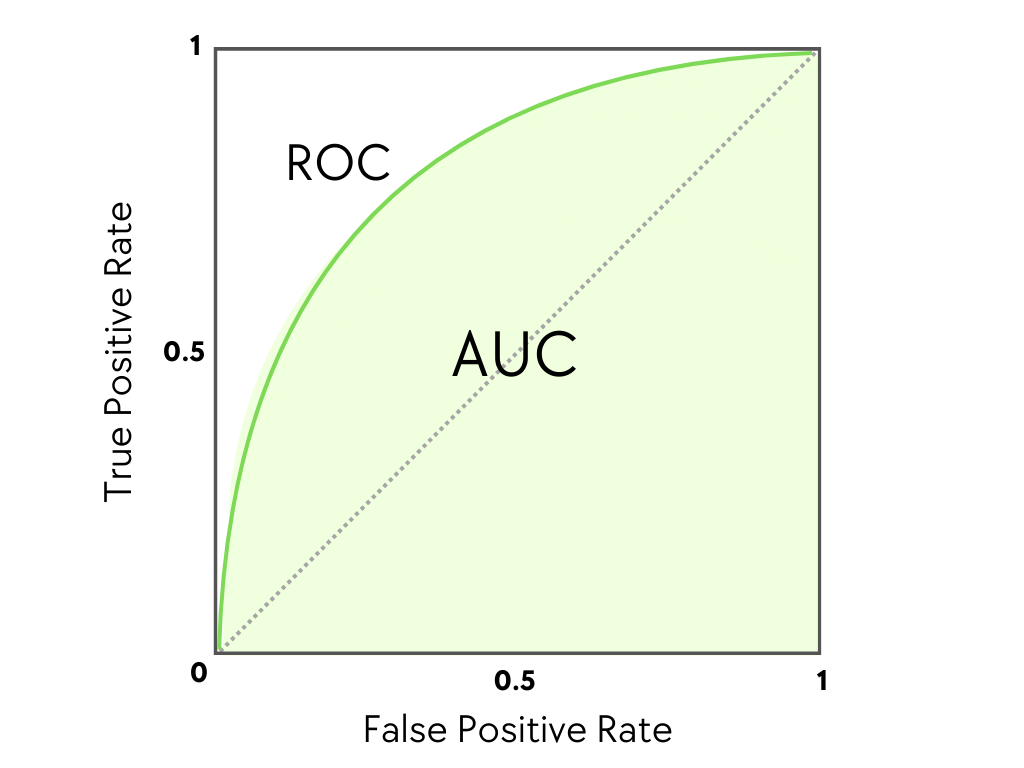
\includegraphics[width=0.4\linewidth]{images/auc_roc_curve.png}
    \end{figure}
\end{frame}

\section{Multiple Logistic Regression}
\subsection{Multiple Logistic Regression}
% Slide 19: Introduction to Multiple Logistic Regression
\begin{frame}{Multiple Logistic Regression}
    \textbf{Extending Logistic Regression to Multiple Predictors}
    \begin{itemize}
        \item In multiple logistic regression, we model the probability of a binary outcome using multiple predictors.
        \item The model equation is:
        \begin{equation}
            \log \left( \frac{p(X)}{1 - p(X)} \right) = \beta_0 + \beta_1 X_1 + \beta_2 X_2 + \dots + \beta_p X_p
        \end{equation}
        \item This allows us to account for multiple factors simultaneously when predicting an outcome.
        \item Model evaluation methods are the same as from simple Logistic Regression.
    \end{itemize}
\end{frame}

% Slide 20: Example of Multiple Logistic Regression
\subsection{Example}
\begin{frame}{Example: Predicting Credit Default}
    \textbf{Using Multiple Predictors:}
    \begin{itemize}
        \item Consider a dataset where we predict whether a person defaults on a loan.
        \item Predictors: Credit balance, income, and student status.
        \item Fitted model:
        \begin{equation}
            \log \left( \frac{p(X)}{1 - p(X)} \right) = -10.869 + 0.0057 \times \text{Balance} + 0.0030 \times \text{Income} - 0.6468 \times \text{Student}
        \end{equation}
        \item Interpretation:
        \begin{itemize}
            \item A one-unit increase in balance increases the log-odds of default.
            \item Being a student decreases the probability of default, holding other factors constant.
        \end{itemize}
    \end{itemize}
\end{frame}

% Slide 21: Interpreting Multiple Logistic Regression Coefficients
\subsection{Interpretation}
\begin{frame}{Interpreting Coefficients}
    \textbf{Understanding the Impact of Each Predictor:}
    \begin{itemize}
        \item \textbf{Odds Ratio:} The exponentiated coefficient \( e^{\beta} \) represents the multiplicative change in the odds.
        \item Example:
        \begin{equation}
            e^{0.0057} \approx 1.0057
        \end{equation}
        \item This means that for each additional dollar in balance, the odds of default increase by approximately 0.57\%.
        \item Similarly, a student has lower odds of default by a factor of:
        \begin{equation}
            e^{-0.6468} \approx 0.523
        \end{equation}
        \item This means students are about 48\% less likely to default than non-students, controlling for other factors.
    \end{itemize}
\end{frame}
\section{Multinomial Logistic Regression}
\subsection{Multinomial Logistic Regression}
% Slide 23: Introduction to Multinomial Logistic Regression
\begin{frame}{Multinomial Logistic Regression}
    \textbf{Extending Logistic Regression to More than Two Classes (Outcomes)}
    \begin{itemize}
        \item When the response variable has more than two categories, multinomial logistic regression is used.
        \item Unlike binary logistic regression, we model multiple class probabilities simultaneously.
        \item The model equation for class \( k \) is:
        \begin{equation}
            P(Y = k | X) = \frac{e^{\beta_{k0} + \beta_{k1}X_1 + \dots + \beta_{kp}X_p}}{\sum_{l=1}^{K} e^{\beta_{l0} + \beta_{l1}X_1 + \dots + \beta_{lp}X_p}}
        \end{equation}
    \end{itemize}
\end{frame}
\subsection{Example}
% Slide 24: Example of Multinomial Logistic Regression
\begin{frame}{Example: Predicting Disease Type}
    \textbf{Classifying Patients into One of Three Conditions:}
    \begin{itemize}
        \item Response Variable: \( Y \) (Disease type: Stroke, Drug Overdose, Epileptic Seizure).
        \item Predictors: Age, Blood Pressure, Medical History.
        \item A fitted model:
        \begin{equation}
            \log \left( \frac{P(Y = \text{Stroke} | X)}{P(Y = \text{Epileptic Seizure} | X)} \right) = \beta_0 + \beta_1 X_1 + \beta_2 X_2
        \end{equation}
        \item Interpretation:
        \begin{itemize}
            \item A one-unit increase in \( X_1 \) (e.g., blood pressure) changes the log-odds of having a stroke relative to an epileptic seizure.
            \item Probabilities for all categories sum to one.
        \end{itemize}
    \end{itemize}
\end{frame}

\subsection{Interpretation}
% Slide 25: Interpreting Multinomial Logistic Regression Coefficients
\begin{frame}{Interpreting Coefficients}
    \textbf{Understanding the Impact of Each Predictor:}
    \begin{itemize}
        \item Coefficients describe log-odds of one category relative to the baseline category.
        \item The exponentiated coefficient \( e^{\beta} \) represents the change in odds for a one-unit increase in the predictor.
        \item Example:
        \begin{equation}
            e^{0.3} \approx 1.35
        \end{equation}
        \item This means that for each unit increase in the predictor, the odds of belonging to a given class (e.g., Stroke) relative to the baseline increase by 35\%.
    \end{itemize}
\end{frame}


\end{document}
